\documentclass[10pt]{amsart} 


\usepackage{amsmath, amssymb, mathrsfs} 

\usepackage[mathscr]{euscript} 
 
\newlength{\mylength}
\setlength{\mylength}{0.25cm}

\usepackage{enumitem}
\setlist{listparindent=\parindent, itemsep=0cm, parsep=\mylength, topsep=0cm}

\usepackage[final]{todonotes}
\usepackage[final]{showkeys} 

\usepackage[breaklinks=true]{hyperref} 
\usepackage{comment} 

\usepackage{graphicx}

\usepackage{url}

\usepackage{tikz-cd}

\usepackage{amsthm}

\makeatletter
\renewenvironment{proof}[1][\proofname]{\par
	\pushQED{\qed}%
	\normalfont \topsep6\p@\@plus6\p@\relax
	\noindent\emph{#1.} 
	\ignorespaces
}{%
\popQED\endtrivlist\@endpefalse
}
\makeatother

\newtheoremstyle{mythm}% name of the style to be used
{\mylength}% measure of space to leave above the theorem. E.g.: 3pt
{0pt}% measure of space to leave below the theorem. E.g.: 3pt
{\itshape}% name of font to use in the body of the theorem
{0pt}% measure of space to indent
{\bfseries}% name of head font
{.\ }% punctuation between head and body
{ }% space after theorem head; " " = normal interword space
{\thmname{#1}\thmnumber{ #2}\thmnote{ (#3)}}

\newtheoremstyle{myrmk}% name of the style to be used
{\mylength}% measure of space to leave above the theorem. E.g.: 3pt
{0pt}% measure of space to leave below the theorem. E.g.: 3pt
{}% name of font to use in the body of the theorem
{0pt}% measure of space to indent
{\itshape}% name of head font
{.\ }% punctuation between head and body
{ }% space after theorem head; " " = normal interword space
{\thmname{#1}\thmnumber{ #2}\thmnote{ (#3)}}

\theoremstyle{mythm} 
%\newtheorem{thm}[subsubsection]{Theorem}
%\newtheorem*{claim}{Claim}
%\newtheorem*{thm}{Theorem} 
\newtheorem{thm}{Theorem}
\newtheorem{lem}[thm]{Lemma} 
\newtheorem{cor}[thm]{Corollary}
\newtheorem{claim}[thm]{Claim}
\newtheorem{prop}[thm]{Proposition}
%\newtheorem*{mthm}{Main Theorem}

%\newtheorem{prop}[subsubsection]{Proposition} 
%\newtheorem*{prop}{Proposition} 
%\newtheorem*{lem}{Lemma}
%\newtheorem*{klem}{Key Lemma}
%\newtheorem*{cor}{Corollary}

\theoremstyle{definition}
%\newtheorem{defn}[subsubsection]{Definition}
\newtheorem*{defn}{Definition} 
\newtheorem{prob}[thm]{Problem}
%\newtheorem{que}[subsubsection]{Question}

\theoremstyle{myrmk} 
%\newtheorem{rmk}[subsubsection]{Remark}
\newtheorem*{rmk}{Remark}
%\newtheorem{note}[subsubsection]{Note} 
\newtheorem*{ex}{Example}

\newcommand{\nc}{\newcommand} 
\nc{\on}{\operatorname}
\nc{\rnc}{\renewcommand} 

\rnc{\setminus}{\smallsetminus} 

\nc{\wt}{\widetilde}
\nc{\wh}{\widehat} 
\nc{\ol}{\overline} 

\nc{\Frob}{\on{Frob}}
\nc{\Gal}{\on{Gal}}

\nc{\BN}{\mathbb{N}}
\nc{\BZ}{\mathbb{Z}}
\nc{\BQ}{\mathbb{Q}}
\nc{\BR}{\mathbb{R}}
\nc{\BC}{\mathbb{C}}

\nc{\id}{\on{id}}
\nc{\Id}{\on{Id}}
\nc{\Tr}{\on{Tr}}

\nc{\la}{\langle}
\nc{\ra}{\rangle} 
\nc{\lV}{\lVert}
\nc{\rV}{\rVert}
\nc{\mb}{\mathbf}
\nc{\mf}{\mathfrak}
%\nc{\cur}{\mathscr}
\nc{\mc}{\mathscr}

\nc{\ira}{\hookrightarrow}
\nc{\hra}{\hookrightarrow}
\nc{\sra}{\twoheadrightarrow} 

\rnc{\Re}{\on{Re}}

\nc{\coker}{\on{coker}}
\nc{\End}{\on{End}}
\rnc{\Im}{\on{Im}}
%\rnc{\Re}{\on{Re}}

\nc{\Hom}{\on{Hom}}

\DeclareMathOperator*{\argmin}{arg\,min}
\DeclareMathOperator*{\argmax}{arg\,max}

\usepackage{marginnote}
\nc{\acts}{\curvearrowright}

\nc{\Mat}{\on{Mat}}

\newenvironment{cd}{\begin{equation*}\begin{tikzcd}}{\end{tikzcd}\end{equation*}\ignorespacesafterend}

\nc{\pfrac}[2]{\frac{\partial #1}{\partial #2}}
\nc{\e}[1]{\begin{align*} #1 \end{align*}}

\usepackage[margin=1in]{geometry}

\makeatletter
\def\blfootnote{\gdef\@thefnmark{}\@footnotetext}
\makeatother

%\renewcommand*{\arraystretch}{1.4}

\setlength{\parskip}{0.25cm}

\definecolor{myblue}{rgb}{0,0.15,0.45}
\newenvironment{myproof}{\color{myblue}\begin{proof}}{\end{proof}} 


\usepackage{bm}

\usepackage{fancyhdr}
\pagestyle{fancy} 
\fancyhead[L]{James Tao}
\fancyhead[C]{18.06 -- Week 13 Recitation}
\fancyhead[R]{May 12, 2020}
\fancyfoot[C]{}

\newcounter{part-count}
\setcounter{part-count}{0}

\newenvironment{me}[1]{\begin{enumerate}[#1]\setcounter{enumi}{\value{part-count}}}{\setcounter{part-count}{\value{enumi}}\end{enumerate}}

\nc{\myhead}[1]{\noindent\emph{#1}.}


\begin{document}
	\thispagestyle{fancy}
	
	In this last recitation, we will study the simplest Toeplitz matrix which is symmetric but not diagonal. This combines many concepts from this course: eigenvalues and eigenvectors, linear recurrences, infinite dimensional space, linear differential equations. At the end, we discuss the relevance of this example to combinatorics, physics, and neuroscience. 
	
	\section{Quantum numbers} 
	
	Let 
	\[
		M = \begin{pmatrix}
		0 & 1 & 0 & 0 & \cdots \\
		1 & 0 & 1 & 0 & \cdots \\
		0 & 1 & 0 & 1 & \cdots \\
		0 & 0 & 1 & 0 & \cdots \\
		\vdots & \vdots  & \vdots  & \vdots  & \ddots
		\end{pmatrix}
	\]
	be an infinite Toeplitz matrix, i.e.\ $M_{ij} = 1$ if $|i-j| = 1$ and $0$ otherwise. If $\bm{v} = (v_1, v_2, \ldots)$ is an infinite vector, then 
	\[
		M \bm{v} = \begin{pmatrix}
		v_2 \\ v_1 + v_3 \\ v_2 + v_4 \\ v_3 + v_5 \\ \vdots
		\end{pmatrix}
	\]
	Fix $\lambda$ and try to find $\bm{v}$ satisfying $M \bm{v} = \lambda \bm{v}$. This equation translates to the following infinite system of linear equations: 
	\e{
		v_2 &= \lambda v_1 \\
		v_3 &= \lambda v_2 - v_1 \\
		v_4 &= \lambda v_3 - v_2 \\
		v_5 &= \lambda v_4 - v_3 \\
		&\ \, \vdots
	} 
	Let $q$ be a solution to $q^2 - \lambda q + 1 = 0$, so that $\lambda = q + q^{-1}$. Then we find that, if $v_1 = 1$, we have 
	\e{
		v_2 &= q + q^{-1} \\
		v_3 &= q^2 + 1 + q^{-2} \\
		v_4 &= q^3 + q + q^{-1} + q^{-3} \\
		v_5 &= q^4 + q^2 + 1 + q^{-2} + q^{-4} \\
		& \ \, \vdots
	} 
	and the pattern continues. These are called \emph{quantum numbers}, or \emph{$q$-numbers} for short. Note that the special case $q = 1$ (corresponding to eigenvalue $\lambda = 2$) corresponds to usual integers, i.e.\ $v_n = n$ for all $n$. 
	
	We have found that every complex number $\lambda$ is an eigenvalue for the infinite Toeplitz matrix $M$. The entries of the corresponding eigenvector are the $q$-numbers, where $q + q^{-1} = \lambda$. 
	
	\myhead{Exercise} Check the relation $v_{k-1} + v_{k+1} = v_2v_k$.
	
	This is a `$q$-analogue' of the ordinary identity $(k-1) + (k+1) = 2k$, which is obtained by setting $q = 1$. 
	
	\newpage
	
	\section{Waves} 
	
	Let $M_n$ be the $n \times n$ analogue of the infinite matrix $M$, obtained by taking its top-left $n \times n$ block. Because $M_n$ is real symmetric, we expect it to have an orthonormal basis of eigenvectors. What are they? 
	
	Let $\bm{v} = (v_1, v_2, \ldots)$ be an eigenvector of $M$ with eigenvalue $\lambda$. If $v_{n+1} = 0$, then we have 
	\e{
		v_2 &= \lambda v_1 \\
		v_3 &= \lambda v_2 - v_1 \\
		& \ \, \vdots \\
		v_n &= \lambda v_{n-1} - v_{n-2} \\
		0 &= \lambda v_n - v_{n-1}, 
	} 
	and these equations imply that $(v_1, v_2, \ldots, v_n)$ is also an eigenvector of $M_n$ with eigenvalue $\lambda$. 
	
	How can we choose $q$ (hence $\lambda$) to ensure $v_{n+1} = 0$? We have 
	\e{
		v_{n+1} &= q^{n} + q^{n-2} + \cdots + q^{-n} \\
		&= \frac{q^{n+1} - q^{-n-1}}{q-q^{-1}},
	} 
	and this equals 0 whenever $q^{2n+2} = 1$ but $q^2 \neq 1$. Thus $q = e^{\frac{2 \pi i k}{2n+2}}$ for some integer $k$. For these special values of $q$, we can explicitly compute the entries of $\bm{v}$, as follows: 
	\e{
		v_r &= \frac{q^{r} - q^{-r}}{q-q^{-1}} \\
		&= \frac{e^{\frac{2\pi i k r}{2n+2}} - e^{\frac{- 2\pi i k r}{2n+2}}}{e^{\frac{2\pi i k}{2n+2}} - e^{\frac{-2\pi i k}{2n+2}}} \\
		&= \frac{\sin(\tfrac{\pi kr}{n+1})}{\sin(\tfrac{\pi k}{n+1})}. 
	} 
	Rescaling by the common denominator $\sin(\tfrac{\pi k}{n+1})$, we conclude that, if $(v_1, \ldots, v_n)$ is defined by 
	\[
		v_r = \sin(\tfrac{\pi kr}{n+1})
	\]
	for $r = 1, \ldots, n$, then it is an eigenvector of $M_n$ with eigenvalue $\lambda = q + q^{-1} = 2 \cos(\frac{\pi k}{n+1})$. 
	
	This gives $n$ independent eigenvectors (with distinct eigenvalues), by taking $k = 1, 2, \ldots, n$. 
	
	The eigenvectors look like waves. Here are the first three eigenvectors for $n = 10$, produced by taking $k = 1,2, 3$, respectively: 
	\begin{center}
		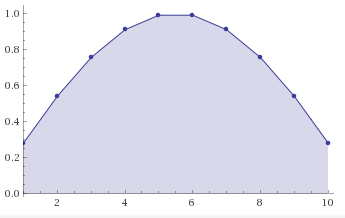
\includegraphics{rec11-pic1}
		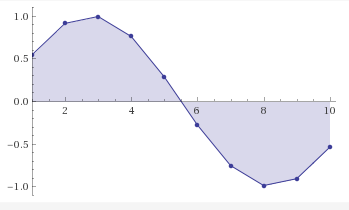
\includegraphics{rec11-pic2}
		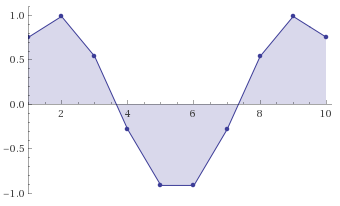
\includegraphics{rec11-pic3}
	\end{center}
	
	The eigenvalue equation $(M_n - 2\on{Id}) \bm{v} = \lambda \bm{v}$ can be viewed as a discretized version of the differential equation $\frac{d^2}{dx^2}\, f(x) = \lambda f(x)$ whose solutions are waves: $f(x) = \sin(x \sqrt{\lambda})$. Under the boundary conditions $f(0) = f(1) = 0$, we see that the only solutions are $f(x) = \sin(xk)$, corresponding to $\lambda = k^2$. 
	
	For comparison, here are these solutions for $k = 1, 2, 3, 100$: 
	\begin{center}
		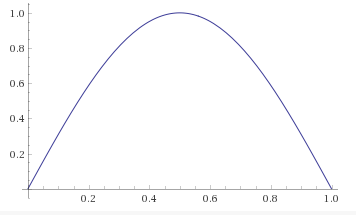
\includegraphics{rec11-pic4}
		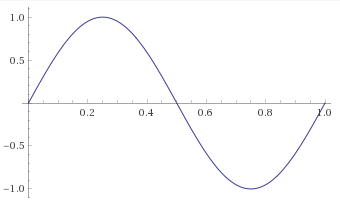
\includegraphics{rec11-pic5}
		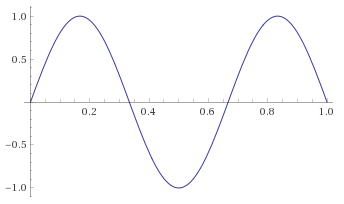
\includegraphics{rec11-pic6}
		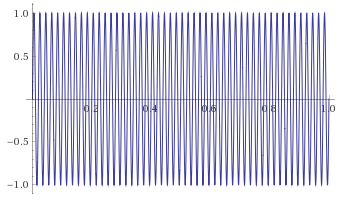
\includegraphics{rec11-pic7}
	\end{center}
	
	\section{Summary and further comments} 

	\begin{itemize}
		\item An infinite matrix (such as $M$) acting on an infinite dimensional vector space can have infinitely many eigenvalues. We saw that every complex number is an eigenvalue of $M$. 
		\item The $q$-numbers allow you to generalize many constructions (and identities) involving ordinary integers, especially those involving factorials and binomial coefficients. 
		\item By truncating $M$ to obtain $M_n$, we forced $q$ to be a $(2n+2)$-nd root of unity. This is a `quantization' phenomenon. The resulting $n$ orthonormal eigenvectors looked like waves. Since they are a basis, any vector in $\BR^n$ can be uniquely expressed as a linear combination of these eigenvectors. This is a discrete version of the Fourier transform. 
		\item The continuous analogue is the differential equation $\frac{d^2}{dx^2} \, f(x) = \lambda f(x)$ with $f(0) = f(1) = 0$. This has an infinite set of solutions, indexed by positive integers, with higher integers giving higher frequencies. Sampling a signal at a constant rate makes very high frequencies look indistinguishable from lower ones: the functions 
		\[
			\sin(\tfrac{\pi k x}{n+1}) \quad \text{and} \quad \sin(\tfrac{\pi (k + 2(n+1)) x}{n+1}) 
		\]
		are very different but agree when $x$ is an integer. This explains why $\frac{d^2}{dx^2}$ has infinitely many eigenvectors but $M_n$ has only finitely many. 
		
		For this reason, in signal processing, one has to choose the sampling rate based on the frequencies one wishes to distinguish. 
		
		In physics, discretizing space (or time) is one way to tame quantities which would otherwise be infinite due to the contribution of arbitrarily high frequencies (e.g.\ `ultraviolet catastrophes'). One studies the behavior of a discretized system (a.k.a.\ `lattice system') as the grid spacing goes to zero. 
		\item The action of the matrix 
		\[
			T := 2 \mathrm{Id} - M_n = \begin{pmatrix}
			2 & -1 & 0 & 0 \\
			-1 & 2 & -1 & 0 \\
			0 & -1 & 2 & -1 \\
			0 & 0 & -1 & 2 
			\end{pmatrix}
		\]
		($n = 4$ case shown) on $\BR^n$ is a simple case of a \emph{center-surround receptive field}, which usually is the first layer of a convolutional neural network that is tasked with image recognition. 
		
		The product $T\bm{u}$ records the dot product of $(-1, 2, -1)$ with all $3$-vectors built by taking three (or fewer) consecutive entries of $\bm{u}$. The word `convolutional' refers to this procedure: choose vector such as $(-1, 2, -1)$ and define a linear transformation by dotting against `all translates' of this vector. Thus, Toeplitz matrices correspond to `convolutional' linear transformations. 
		
		The purpose of the center-surround receptive field is to do edge detection: for example, 
		\[
			T \begin{pmatrix}
			0 \\ 0 \\ 0 \\ 0 \\ 1 \\ 1 \\ 1 \\ 1
			\end{pmatrix} = \begin{pmatrix}
			0 \\ 0 \\ 0 \\ -1 \\ 1 \\ 0 \\ 0 \\ 0
			\end{pmatrix} \quad \text{and} \quad T \begin{pmatrix}
			1 \\ 2 \\ 3 \\ 4 \\ 5 \\ 6 \\ 7 \\ 8
			\end{pmatrix} = \begin{pmatrix}
			0 \\ 0 \\ 0 \\ 0 \\ 0 \\ 0 \\ 0 \\ 9 
			\end{pmatrix}
		\]
		The nonzero entries of $T\bm{u}$ show you where the `sharp' changes in $\bm{u}$ occur. 
		
		Our eigenvector analysis shows that low-frequency wave patterns are suppressed, while high-frequency wave patterns are amplified. This makes sense because high-frequency wave patterns look like `edges.' 
	\end{itemize}
	
	
	
	
	
	
	
\end{document} 